\chapter[Análise de Requisitos]{Análise de Requisitos globais}

Neste capítulo explicaremos o proceso de análise de requisitos levado a cabo para a contrución da ferramenta.

\section{Consultas cos traductores}
Para facer unha nova ferramenta de asistencia a tradución consultamos os usuarios principais da ferramenta. Para iso enviamos correos as unhas cantas listas de correo de traductores de diferentes proxectos de software libre como os seguintes:

\paragraph{GNOME} Dentro do proxecto GNOME hai un grupo especifico para a internacionalización dos programas da plataforma. Existen listas de correo para cada linguaxe e unha a nivel internacional. En concreto as listas que enviamos un correo preguntando por ideas para o novo programa foron a lista \emph{internacional}, a lista de traductores o \emph{galego} e a lista de traductores ao \emph{castelán}.

\paragraph{Proxecto Trasno} É unha comunidade de traductores de proxectos de software libre ao Galego. Sirve de punto de encontro para os traductores galegos e realiza periodicamente reunións para a discursión da terminoloxía a usar e a presentación de novas ferramentas.

\paragraph{OpenSuse e Fedora} Estas dúas distribucións de Linux contan cos seus respectivos equipos de traductores. Aínda que a maior parte dos programas destas distribucións son traducidos por outros proxectos, como pasa no caso do entorno de escritorio GNOME, si que hai partes do sistema que necesitan ser traducidas polos propios traductores de cada distribución.

\paragraph{OpenOffice e LibreOffice} Tanto OpenOffice como o seu \emph{fork}, LibreOffice, contan con equipos internacionalización aos que se lles consultou para recoller ideas para o novo programa.

\paragraph{Mozilla} O proxecto Mozilla, autores do navegador Firefox e do xestor de correo electrónico Thunderbird, conta cun equipo de traductores propio. Neste caso non usan ficheiros de tipo Gettext PO, senon ficheiros XML.

Case en todos os correos enviados houbo xente que respondeu dando ideas sobre o que lles gustaría que incorporase o novo programa. Na seguinte sección podemos ver a maioría destas utilidades explicadas.

\subsection{Resumo das peticións}
	\paragraph{Abrir e gardar ficheiros en diferentes formatos.} O programa debería permitir abrir outros formatos de ficheiros aparte do formato Gettext po. Esta petición foi feita sobretodo por membros de equipos de tradutores que non son de GNOME. Existe unha biblioteca de nome \emph{translate-toolkit} que facilita a conversión entre formatos.

	\paragraph{Xestión de cabeceiras} Que o programa modifique automaticamente as cabeceiras con metainformación que tanto o formato Gettext PO como outros tipos de formatos teñen.

	\paragraph{Perfiles de usuarios} Permitir ter diversos perfiles de usuarios para diferentes proxectos de tradución ou para diferentes linguaxes.

	\paragraph{Vista de proxecto} Os traductores consideran moi interesante agrupar os ficheiros relacionados en proxectos e poder ter estatísticas de proxectos.

	\paragraph{Buscar e buscar e reemplazar}  Regex, search in several files/ in the whole document, update translation files with new ones.

	\paragraph{Dividir/Misturar ficheiros} Os traductores consideran que é interesante que en ficheiros grandes exista a posibilidade de dividir e volver a unir ficheiros de tradución para que así sexa posible que máis dunha persona traballe no mesmo ficheiro a vez.

	\paragraph{Medidas Económicas} É interesante incorporar unha ferramenta que permita calcular o custe da tradución efectuada por un traductor. Istó é especialmente util cando falamos de traductores profesionais e non amateur.

	\paragraph{Resaltado da síntaxe} O programa debe resaltar aqueles elementos da cadea que non son traducibles e pertencen o dominio das linguaxes de programación. Por exemplo na seguinte cadea \lstinline[language=C]{"Temos %i coches."} o elemento \lstinline[language=C]{%i} debería estar resaltado xa que so parte do formateado da cadea por parte do programa.

	\paragraph{Comunicación con servidor web} Os traductores consideran a posiblididade de que o porgrama permita certa comuniación con xestores de traducións en internet. No caso de GNOME o programa Damned Lies xestiona os ficheiro .po para todolos programas de GNOME e os traductores deben baixar e subir os ficheiros dende esa plataforma.

	\paragraph{Navegación dentro do documento} A posibilidade de navegar a través das cadeas. Engadir a posibilidade de ir a seguinte cade traducida, sen traducir ou con unha tradución difusa.

	\paragraph{Memoria de tradución} Engadir unha memoria de tradución que permita exportar e importar ficheiros en diferentes formatos. Ter varias memorias  de tradución con prioridade entre elas, engadir a posibilidade de editar a meoria de tradución e acceder a diversos servidores que xestionan memorias de tradución online como poden ser Trobador, amaGama, Open-tran ou Transvision. Import/Export different formats (.po, .tmx, …) Several TM. Priority. Update a TM., TMX Server (Trobador, amaGama, Open-tran and Transvision),

	\paragraph{Glosario} Engadir a posibilidade de consultar a tradución de termos contra ficheiros unha base de datos local ou contra un servidor de glosario como pode ser Terminator.

	\paragraph{Busca de termos} Que o programa permita a busqueda nun dicionario tanto local como en internet. Citanse dicionarios en internet como o que proporciona Wikipedia ou a Universidade de Santiago de Compostela para o galego.

	\paragraph{Previsualización das traducións} Moitas das interfaces que se fan actualmente empregan ferramentas de cuarta xeneración que permitirían xerar a interfaz cas traducións. No caso de GNOME, Glade é o programa que permite a creación de interfaces e xa existe unha ferramenta online que permite a previsualización de traducións de nome Deckard. O que se pide é que o programa incorpore esa posibilidade dende a súa interface.

	\paragraph{Programa controlable totalmente a través do teclado} O programa en xeral peros sobretodo a interface de edición de ficheiros debe ser manexable totalmente a través do teclado para mellorar a productividade dos traductores. Os traductores piden tamén a posibilidade de que se permita personalizar os atallos de teclado.

	\paragraph{Tradución doutras linguaxes} Hai linguas como o galego e o portugués que se parecen moito polo que as veces resulta moi útil poder, en vez de partir de cero, coller unha tradución dun idioma semellante e editala.

	\paragraph{Comprobacións} Os traductores resaltaron a utilidade de que a ferramenta comprobe certa parametros para comprobar a calidade da tradución. Entre outros:
		\begin{itemize}
			\item \textbf{Ortografía e Gramática.} O programa avisará se a cadea traducida ten erros tanto ortográficos e gramaticais.
			\item \textbf{Coherencia terminolóxica.} O programa avisará o usuario cando este empregue unha tradución dun termo diferente a que se ven empregando no resto do ficheiro.
			\item \textbf{Tags XML e marcas de formato.} O programa avisará o usuario se faltan ou están mal escritos os diferentes tags XML ou marcas de formato.
		\end{itemize}

	\paragraph{Multiplataforma} A aplicación debe estar dispoñible para varios sistemas operativos (BSD, Windows, MAC OS, etc.).

	\paragraph{Tradución automatica} O aplicativo debe incorporar mecanismos de tradución automática emptegando ferramentas como Google Translator, Bing Translator, Opentrad ou Apertium.

	\paragraph{Estatísticas} Débese amosar estatísticas tanto a nivel de ficheiro como de proxecto do numero de cadeas ou palabras traducidas, sen traducir ou difusas.

\section{Análise doutros aplicativos do mercado}
Para facer o novo produto software para a tradución tamén consultamos outras ferramentas similares existentes no mercado para intentar imitar as súas vantaxes e evitar as súas deficiencias. O resultado desta análise pódese consultar na Seccion~\ref{sec:ferramentascat}.

\section{Requisitos do aplicativo}
Con toda a información obtida realizamos unha lista de casos de uso que debe cumplir o programa.

\begin{itemize}
  \item \textbf{Abrir ficheiro.} O programa debe ser capaz de abrir ficheiros PO pero tamén ter un deseño extensible que permita abrir outros formatos.
  \item \textbf{Gardar ficheiro.} Debemos poder gardar ficheiros PO pero tamén ter un deseño extensible que permite gardar noutros formatos.
  \item \textbf{Amosar ficheiro.} Debemos amosar o contido dos ficheiros e dicir, as cadeas e as estatísticas deste ficheiro.
  \item \textbf{Editar ficheiro.} Debemos permitir editar o contido dos ficheiros.
  \item \textbf{Buscar cadeas.} A aplicación permitirá buscar entre as cadeas do ficheiro.
  \item \textbf{Navegar polas cadeas.} Permitiremos navegar polas cadeas do ficheiro podendo avanzar entre as cadeas traducidas, sen traducir, etc.
  \item \textbf{Xestionar perfiles.} Permitiremos xestionar diferentes perfiles para os traductores.
  \item \textbf{Obter pistas.} Amosaremos ao usuario pistas que lle indequen que está a facer algo mal.
  \item \textbf{Obter suxerencias.} Debemos amosar ao tradutor diferentes alternativas de traducións.
\end{itemize}

Na figura~\ref{fig:casosdeuso} podemos ver o Diagrama UML de casos de uso para este programa.

\begin{figure}[h!]
    \centering
    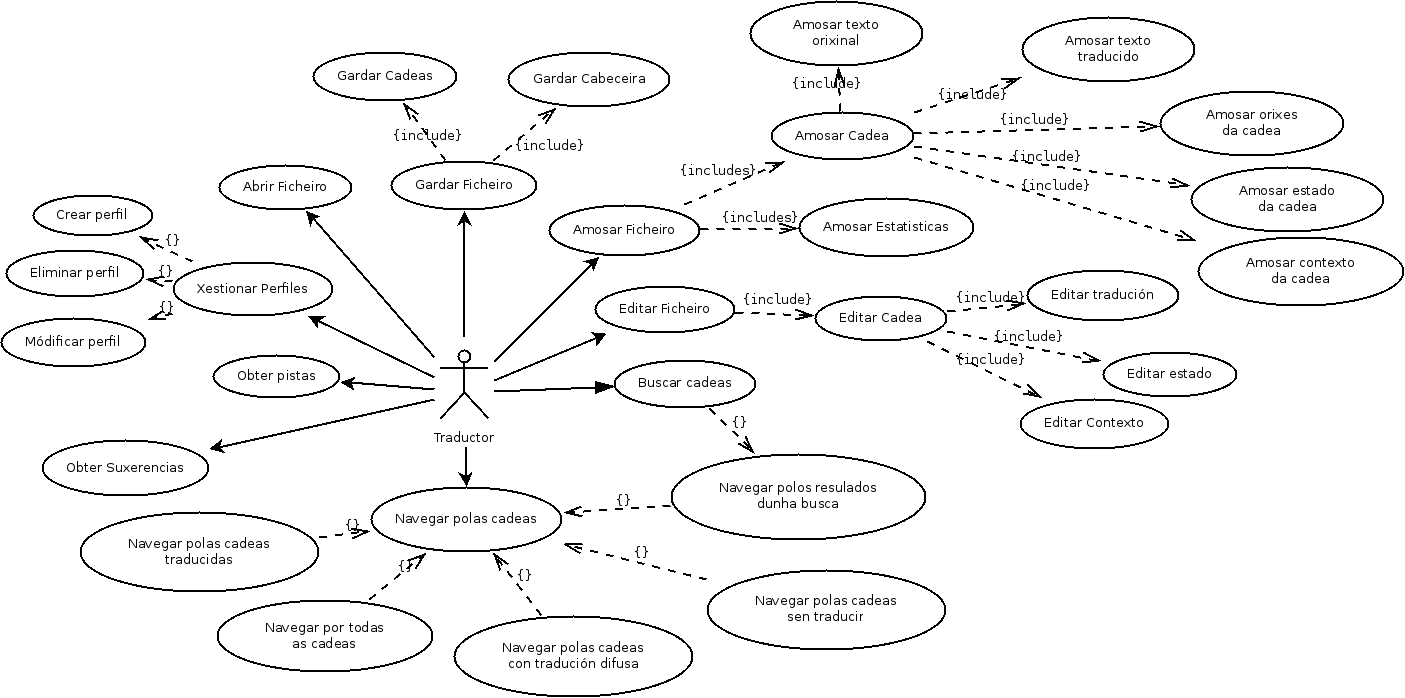
\includegraphics[width=0.9\textheight,angle=90]{img/casosdeuso.png}
    \caption{Diagrama UML de casos de uso do aplicativo}
    \label{fig:casosdeuso}
\end{figure}

%
% FIN DEL CAPÍTULO
%
